\subsection{Decomposition of $d(K^-, N)"\pi\Sigma"$ spectra}

In this subsection, we decompose the obtained spectra into $I=0$, $I=1$ and their interference terms, and discuss how each of them affects the spectrum.
Based on the two-step reaction mechanism described so far, the obtained $d(K^-, N)"\pi \Sigma"$ spectrum can be expressed as follows.

\newcommand{\Tmat}{T_{\bar{K}N \rightarrow \pi \Sigma}}
\newcommand{\Cfirst}{C_{K^- N \rightarrow \bar{K}N}}
\begin{align}
  \frac{d\sigma}{d\Omega dM}(\pi^\mp \Sigma^\pm) \propto & \left| \Cfirst^0 \Tmat^{I=0} \mp \Cfirst^1 \Tmat^{I=1} \right|^2 \nonumber \\
   = & \left| \Cfirst^0 \Tmat^{I=0} \right|^2 + \left| \Cfirst^1 \Tmat^{I=1} \right|^2 \nonumber \\
  & \mp 2\mbox{Re}( \Cfirst^0 \Cfirst^1 \Tmat^{I=0} \Tmat^{I=1} ) & \label{eq:Charge_piS} \\
  \frac{d\sigma}{d\Omega dM}(\pi^- \Sigma^0) \propto & \left| \Cfirst^1 \Tmat^{I=1} \right|^2 \label{eq:pimS0}
\end{align}

Here, $\Tmat^{I=0,1}$ is $T$ matrix of second $\bar{K}N \rightarrow \pi \Sigma$ scattering with $I=0, 1$.
And, $\Cfirst^{0, 1}$ represent the factor of first $K^- p \rightarrow \bar{K}N$ scattering about $I=0, 1$ of the second scattering.
These are complex values that depend on the total energy of the scattering and are $\pi\Sigma$ invariant mass in the case of the second scattering.

\begin{figure}[htbp]
  \begin{tabular}{cc}
    \begin{minipage}{0.5\hsize}
      \centering
      \includegraphics[width=6.0cm]{../pic/Dron/comp_kamano_I0.eps}
    \end{minipage}

    \begin{minipage}{0.5\hsize}
      \centering
      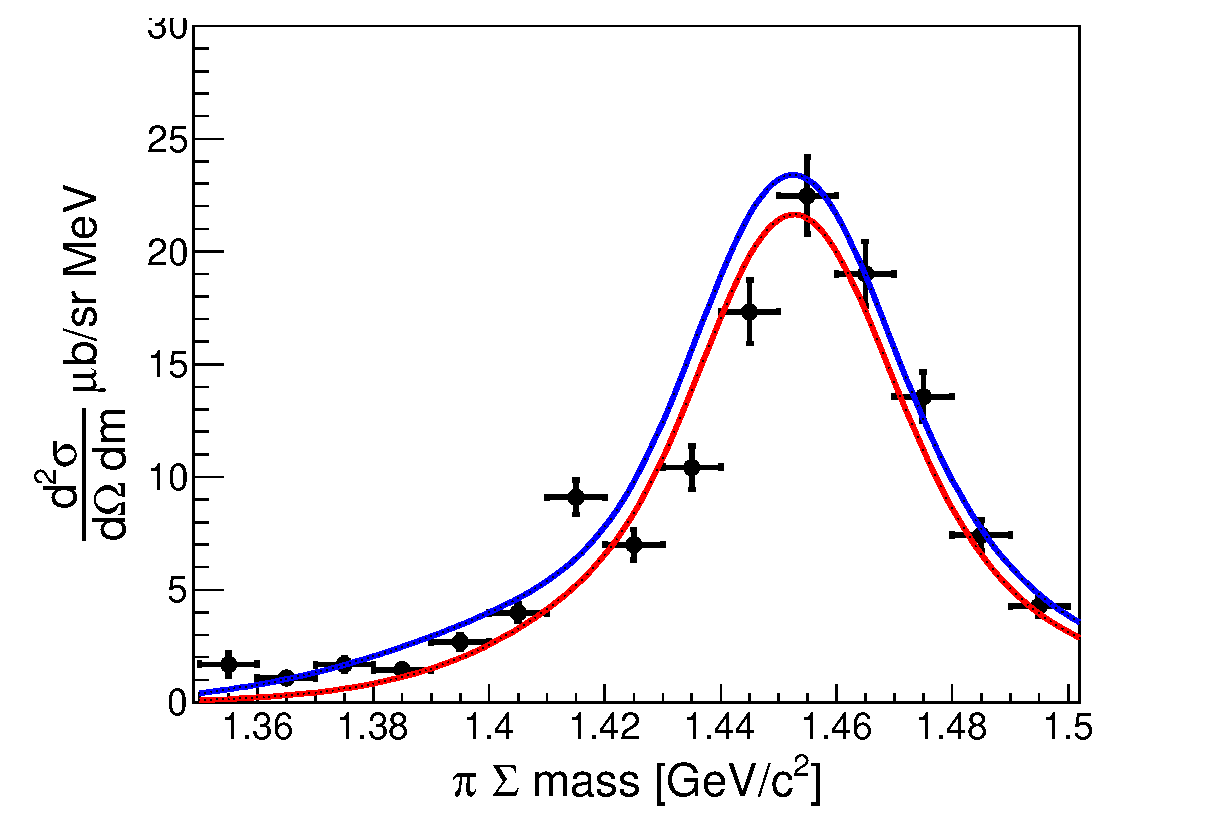
\includegraphics[width=6.0cm]{../pic/Dron/comp_kamano_interfer.eps}
    \end{minipage}
  \end{tabular}

  \centering
  \includegraphics[width=6.0cm]{../pic/Dron/comp_kamano_I1.eps}
  \caption{
    These figures show a comparison between our data and theoretical calculations of the DCC models (models.A and model.B).
    The black error bars represent our data.
    The blue and red lines represent Model.A and Model.B respectively.
    The top right figure shows the strength of $I=0$, the top left figure shows the interference term and the bottom figure shows the strength of $I=1$.
  }
  \label{fig:decomposed_DCC}
\end{figure}

\begin{table}[h]
  \caption{
    This table shows the pole position with $I=0$ and $J^P=1/2^-$ below the $\bar{K}N$ threshold by DCC models\cite{DCC2}
  }
  \centering
  \begin{tabular}{ccc}
    \hline
    \hline
    & pole1 & pole2 \\
    \hline
    Model.A & $1437-75i$ & $1372-56i$ \\
    Model.B & $1428-31i$ & $1397-98i$ \\
    \hline
    \hline
  \end{tabular}
  \label{table:DCC_poles}
\end{table}


Figure.\ref{fig:decomposed_DCC} shows the decomposition into $I = 0$, $I = 1$, and their interference terms according to Eq.(\ref{eq:Charge_piS}, \ref{eq:pimS0}).
For comparison, the same procedure for the spectra predicted from the DCC model is also plotted.

These are discussed in turn.
First, the interference term are in good agreement with our experimental values for both Model.A and Model.B.

Second, for $I=1$, the spectral shape strongly reflects the quasi-elastic scattering, which is consistent with both Model.A and Model.B. 
However, the strength of Model.A is less than our experimenta data.

Next, consider the $I=0$ channel, which reflects the effect of $\Lambda(1405)$.
For Model.A, the spectral shape seems to reproduce our experimental data well, although the overall strength is somewhat larger.
On the other hand, Model.B has a long tail below the $\bar{K}N$ threshold and this part does not match the spectral shape of our experiment.

Model .A has a large width at the higher pole that is strongly reflected in this response as shown in Table.\ref{table:DCC_poles},
thus Model.A has a large tail component below the $\bar{K}N$ threshold.

In the next subsection, we discuss how these components affect the spectra by parameterizing them by the scaling factor of each component of the DCC model.


